\documentclass{beamer}
\usepackage[utf8]{inputenc}

\usetheme{Madrid}
\usecolortheme{default}
\usepackage{amsmath,amssymb,amsfonts,amsthm}
\usepackage{txfonts}
\usepackage{tkz-euclide}
\usepackage{listings}
\usepackage{adjustbox}
\usepackage{array}
\usepackage{tabularx}
\usepackage{gvv}
\usepackage{lmodern}
\usepackage{circuitikz}
\usepackage{tikz}
\usepackage{graphicx}

\setbeamertemplate{page number in head/foot}[totalframumber]

\usepackage{tcolorbox}
\tcbuselibrary{minted,breakable,xparse,skins}

\definecolor{bg}{gray}{0.95}
\lstset{
    language=C,
    basicstyle=\ttfamily\small,
    keywordstyle=\color{blue},
    stringstyle=\color{orange},
    commentstyle=\color{green!60!black},
    numbers=left,
    numberstyle=\tiny\color{gray},
    breaklines=true,
    showstringspaces=false,
}

%------------------------------------------------------------
\title{4.13.16}
\date{October 4,2025}
\author{EE25BTECH11011 - Navya Banavathu}
\usepackage{multicol}
\begin{document}

\frame{\titlepage}

\begin{frame}{Question}
 The lines $p(p^2+1)x - y+q=0$and $(p2+1)^2 x+(p^2+1) y+2q=0$ are perpendicular to a common line for
\begin{enumerate}
\begin{multicols}{2}
    \item exactly one value of p
    \item exactly two values of p
    \item more than two values of p 
    \item no value of p
    \end{multicols}
\end{enumerate}
\end{frame}

\begin{frame}{Solution}
Given lines are,
\begin{align}
& p(p^2+1)x - y + q = 0  \\
& (p^2+1)^2 x + (p^2+1)y + 2q = 0
\end{align}

The normal vectors of the lines are
\begin{align}
\vec{n_1} &= \begin{pmatrix} p(p^2+1)\\ -1 \end{pmatrix}, \quad
\vec{n_2} = \begin{pmatrix} (p^2+1)^2 \\ p^2+1 \end{pmatrix}
\end{align}
\end{frame}

\begin{frame}{Solution}
If both lines are perpendicular to a common line with normal vector $\vec{m}$, then
\begin{align}
\vec{n_1}^T \vec{m} &= 0, \\
\vec{n_2}^T \vec{m} &= 0.
\end{align}

This implies $\vec{m}$ lies in the null space of the matrix
\begin{align}
N &= \begin{pmatrix}
\vec{n_1}^T \\
\vec{n_2}^T
\end{pmatrix}
= \begin{pmatrix}
p(p^2+1) & -1 \\
(p^2+1)^2 & p^2+1
\end{pmatrix}.
\end{align}

For a non-trivial solution $\vec{m} \neq 0$ to exist,
\begin{align}
\det(N) = 0.
\end{align}
\end{frame}

\begin{frame}{Solution}
Now,
\begin{align}
\det &= p(p^2+1)(p^2+1) - (-1)\big((p^2+1)^2\big) \\
&= p(p^2+1)^2 + (p^2+1)^2 \\
&= (p+1)(p^2+1)^2
\end{align}

Thus, the condition becomes
\begin{align}
(p+1)(p^2+1)^2=0 \quad\Longrightarrow\quad p=-1 \quad\text{or}\quad p^2+1=0\end{align}

Since $p^2+1=0$ gives nonreal $p$, the only real solution is
\begin{align}
    \boxed{p=-1}
\end{align}
Hence there is exactly one real value of $p$.


\end{frame}

\begin{frame}[fragile]{ Code (C)}
\begin{block}{Part 1}
\begin{lstlisting}[language=C, basicstyle=\ttfamily\small, keywordstyle=\color{blue}, frame=single]
#include <stdio.h>
#include <math.h>

int solve_real_p(double *p_real) {
    int count = 0;
    // Factor 1: (p+1) = 0
    p_real[count++] = -1;
    // Factor 2: (p^2 + 1)^2 = 0 -> p^2 + 1 = 0
    // Check for real roots
    double discriminant = -1;  // p^2 = -1
    if (discriminant >= 0) {
        p_real[count++] = sqrt(discriminant);
        p_real[count++] = -sqrt(discriminant);
    }
    return count;  // number of real roots
}
\end{lstlisting}
\end{block}
\end{frame}


\begin{frame}[fragile]{Python Code}
\begin{block}{Part 1}
\begin{lstlisting}[language=Python, basicstyle=\ttfamily\small, keywordstyle=\color{blue}, frame=single]
import ctypes
import os
import matplotlib.pyplot as plt
import numpy as np

# Step 1: Load the C library
if os.name == "nt":  # Windows
    lib = ctypes.CDLL("./code11.dll")
else:
    lib = ctypes.CDLL("./code11.so")

from ctypes import c_double

lib.solve_real_p.argtypes = [ctypes.POINTER(c_double)]
lib.solve_real_p.restype = ctypes.c_int
\end{lstlisting}
\end{block}
\end{frame}


\begin{frame}[fragile]{Python Code}
\begin{block}{Part 2}
\begin{lstlisting}[language=Python, basicstyle=\ttfamily\small, keywordstyle=\color{blue}, frame=single]
# Array to store real roots
p_real_array = (c_double * 2)()
num_roots = lib.solve_real_p(p_real_array)

# Use the first real root (p = -1)
p = p_real_array[0]
print(f"Real solution from C function: p = {p}")

# Step 2: Define the lines
q = 1  # arbitrary value
x = np.linspace(-5, 5, 400)

# Line equations
y1 = p*(p**2 + 1)*x + q
y2 = -((p**2 + 1)**2 * x + 2*q)/(p**2 + 1)
\end{lstlisting}
\end{block}
\end{frame}

\begin{frame}[fragile]{Python Code: Plotting}
\begin{block}{Part 3}
\begin{lstlisting}[language=Python, basicstyle=\ttfamily\small, keywordstyle=\color{blue}, frame=single]
# Step 3: Common perpendicular
# Slope of perpendicular line: m_perp = 1/2
m_perp = 1 / 2

# Choose a point halfway between the two lines at x=0
y_mid = (y1[200] + y2[200]) / 2
x_perp = np.linspace(-5, 5, 400)
y_perp = m_perp * x_perp + y_mid  # line passing through midpoint

# Step 4: Plot everything
plt.figure(figsize=(7, 5))
plt.plot(x, y1, label='L1: p(p^2+1)x - y + q = 0', color='blue')
plt.plot(x, y2, label='L2: (p^2+1)^2 x + (p^2+1)y + 2q = 0', color='red')
plt.plot(x_perp, y_perp, '--', label='Common perpendicular', color='green')

\end{lstlisting}
\end{block}
\end{frame}

\begin{frame}[fragile]{Python Code: Plotting}
\begin{block}{Part 4}
\begin{lstlisting}[language=Python, basicstyle=\ttfamily\small, keywordstyle=\color{blue}, frame=single]
plt.xlabel('x')
plt.ylabel('y')
plt.title(f'Lines and Common Perpendicular for p = {p}')
plt.grid(True)
plt.legend()
plt.axhline(0, color='black', linewidth=0.8)
plt.axvline(0, color='black', linewidth=0.8)

# Step 5: Save figure
plt.savefig("fig11.png", dpi=300)
plt.show()
\end{lstlisting}
\end{block}
\end{frame}

\begin{frame}{Graphical Representation}
    \begin{figure}
        \centering
        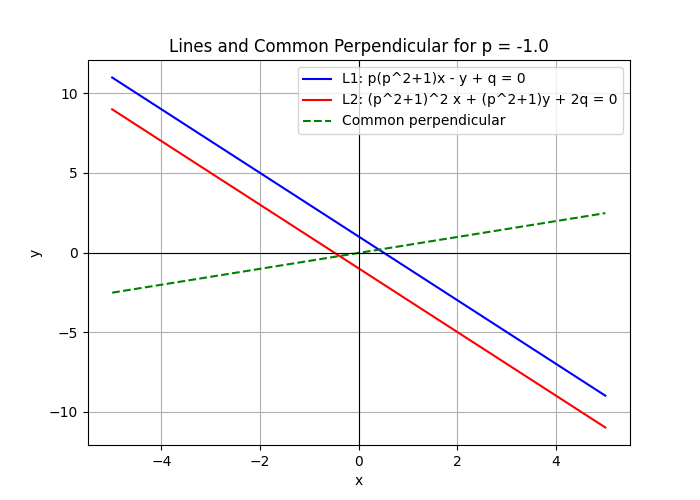
\includegraphics[width=0.6\columnwidth]{../beamer/figs/fig11.png}
    \end{figure}
\end{frame}

\end{document}

